% !TeX spellcheck = fr_FR
\chapter{Chapitre 5 : Analyse des résultats}

Ce chapitre synthétise la qualité des correspondances ATLAS $\leftrightarrow$ OSM. Nous mettons l'accent sur: lecture par méthode, variations par opérateur, couverture par tranches de distance, et cas extrêmes.

\section{Lecture globale par méthode}

\begin{figure}[H]
    \centering
    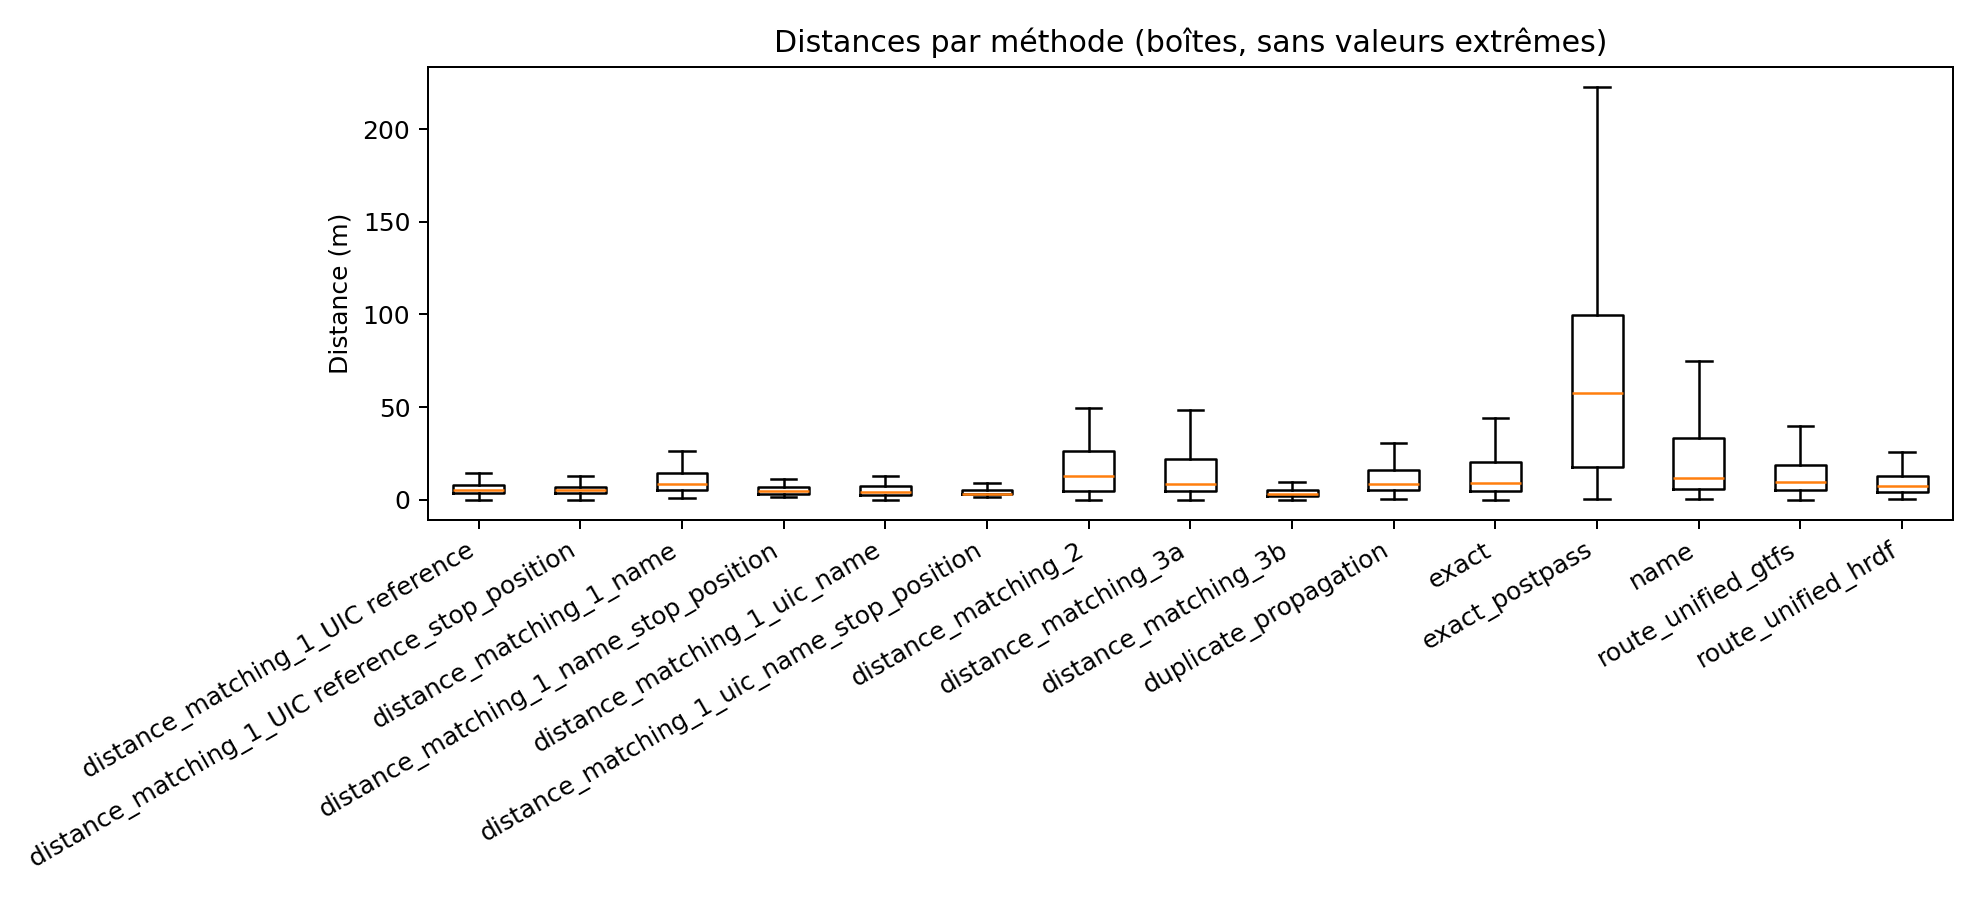
\includegraphics[width=\textwidth]{../figures/chap5/distances_by_method_box.png}
    \caption[Boîtes par méthode]{Boîtes à moustaches par méthode (sans valeurs extrêmes) — médianes et dispersion.}
\end{figure}

\begin{figure}[H]
    \centering
    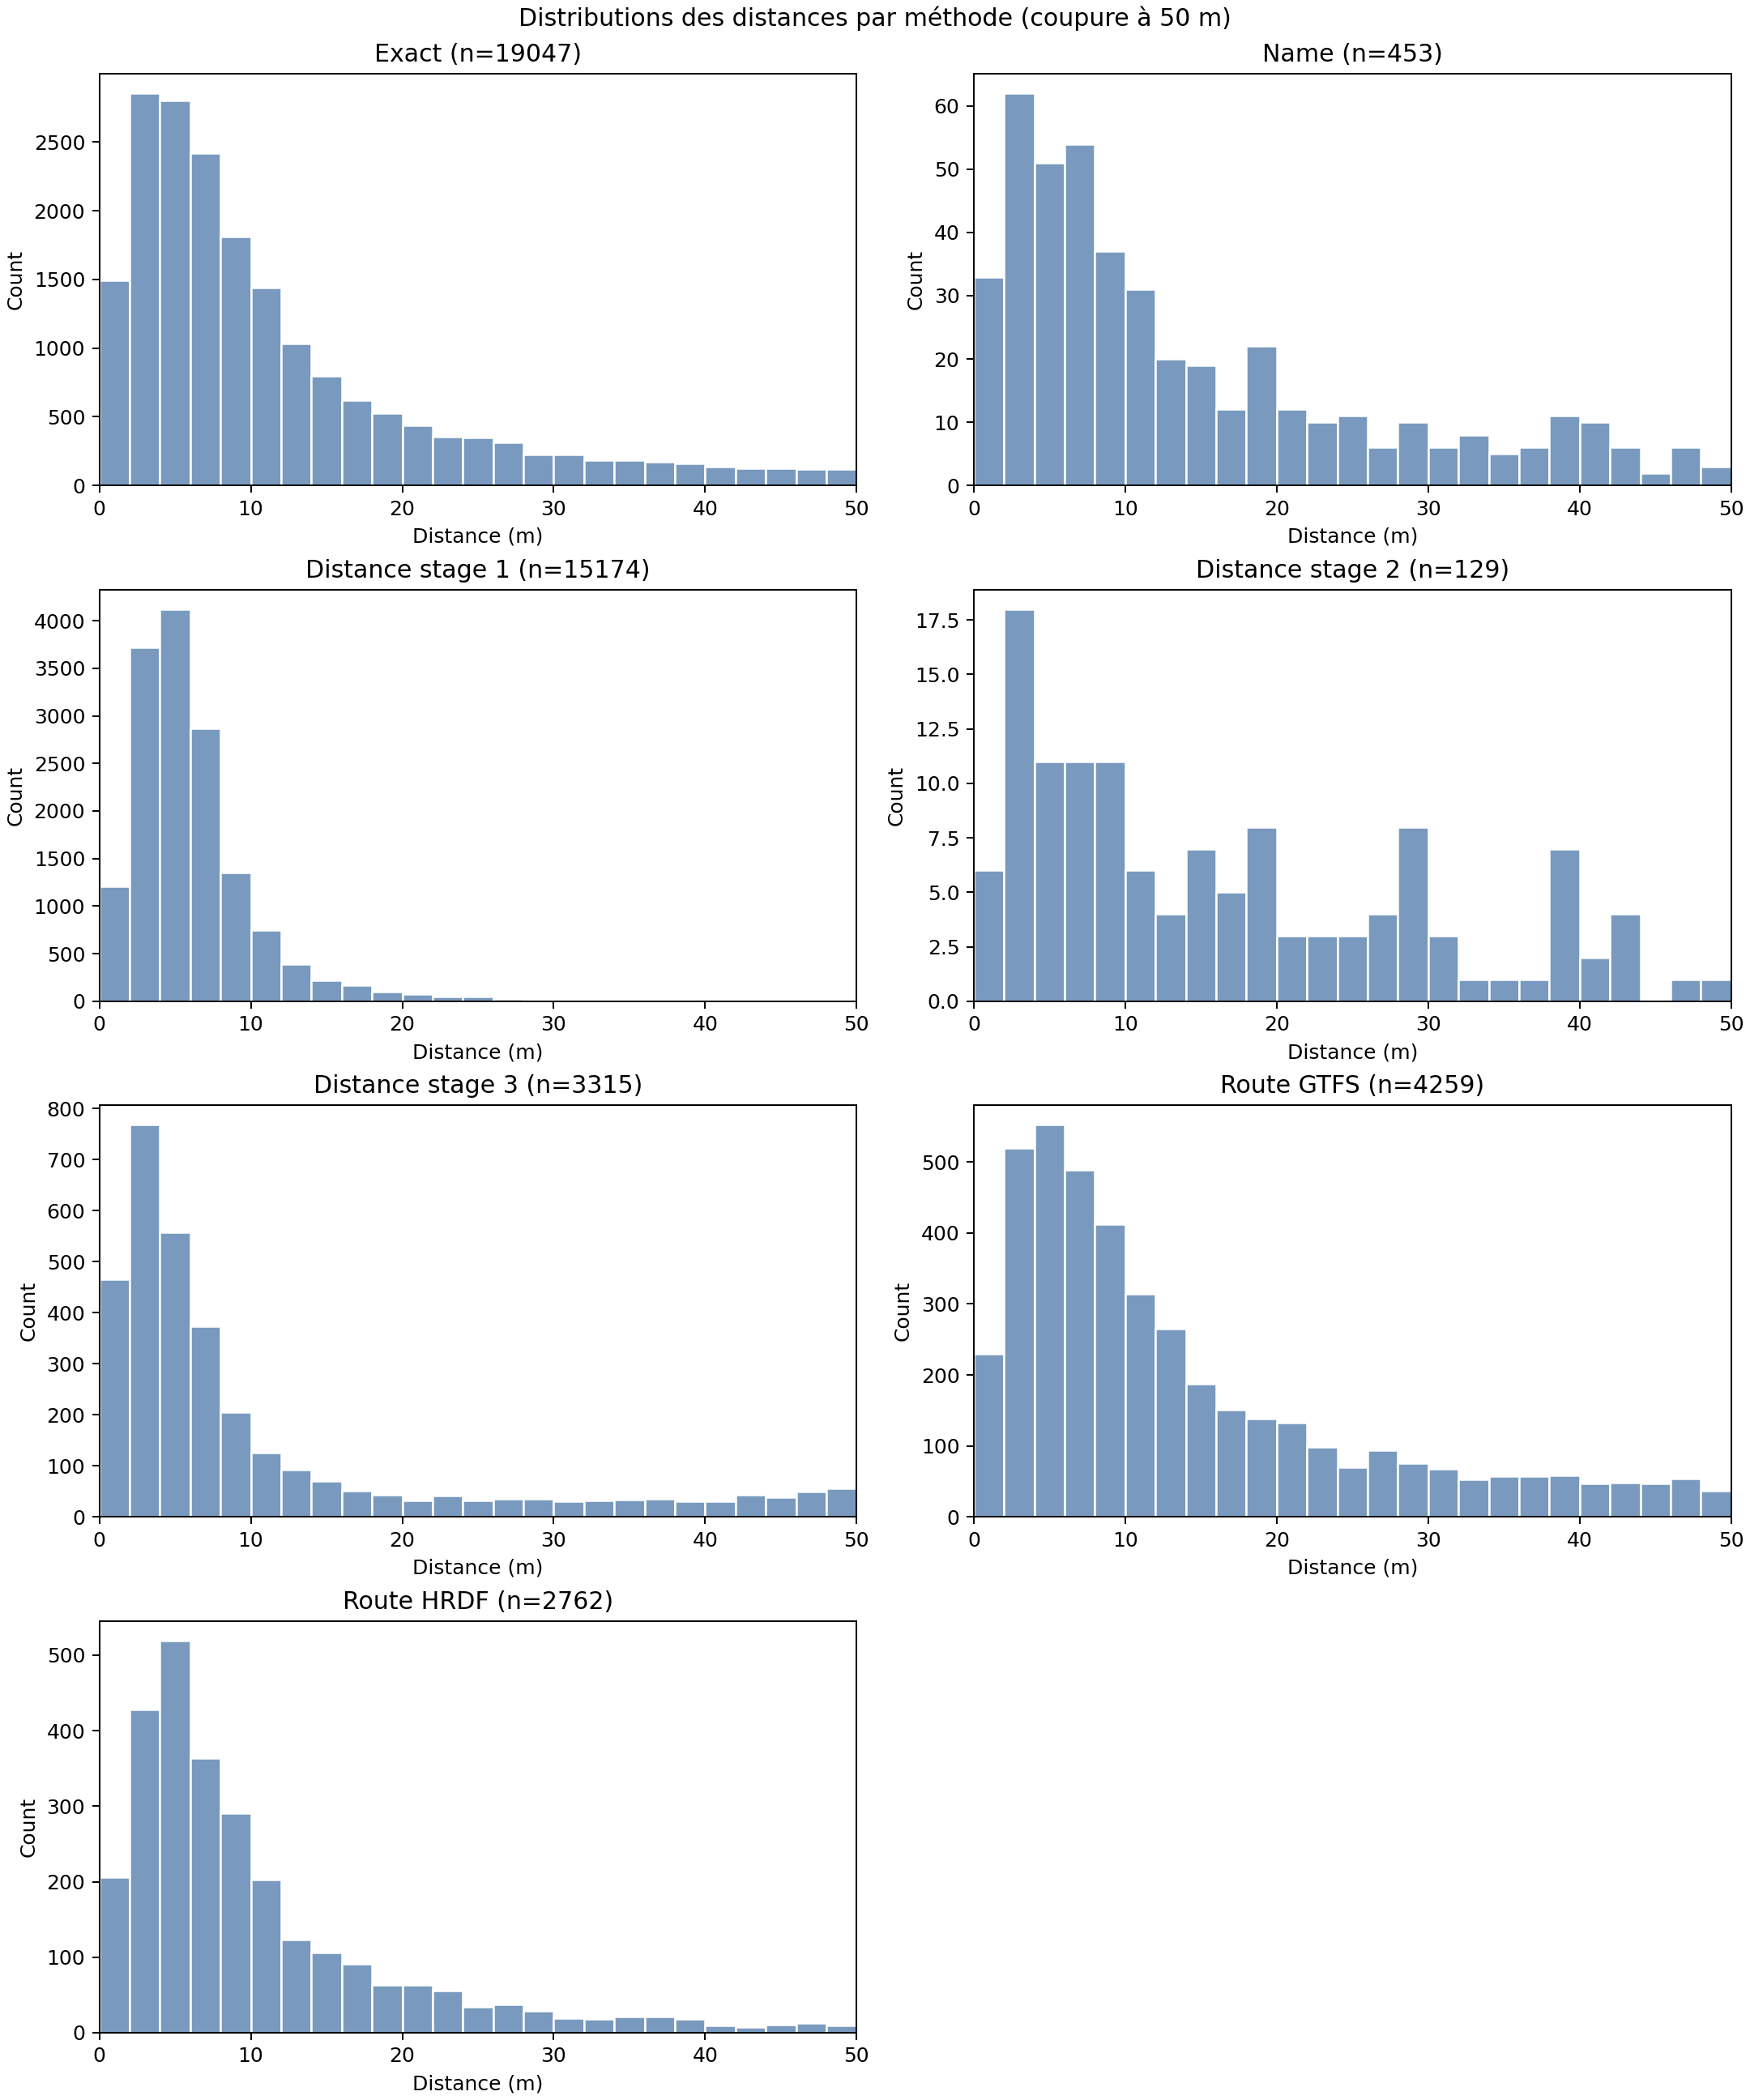
\includegraphics[width=\textwidth]{../figures/chap5/distance_distributions_methods_0_50.png}
    \caption[Histogrammes par méthode (0–50 m)]{Histogrammes des distances coupées à 50 m par méthode: Exact, Name, Distance (stages 1–3), Route GTFS, Route HRDF. Note: sauf Exact et Name, les méthodes de distance et de routes sont par construction limitées à 50 m.}
\end{figure}

\section{Par opérateur: où est-ce le plus précis ?}

Nous relions chaque arrêt à son opérateur ATLAS et observons les distances des arrêts \textit{appariés}. Ci-dessous, la dispersion pour les opérateurs les plus représentés.

\begin{figure}[H]
    \centering
    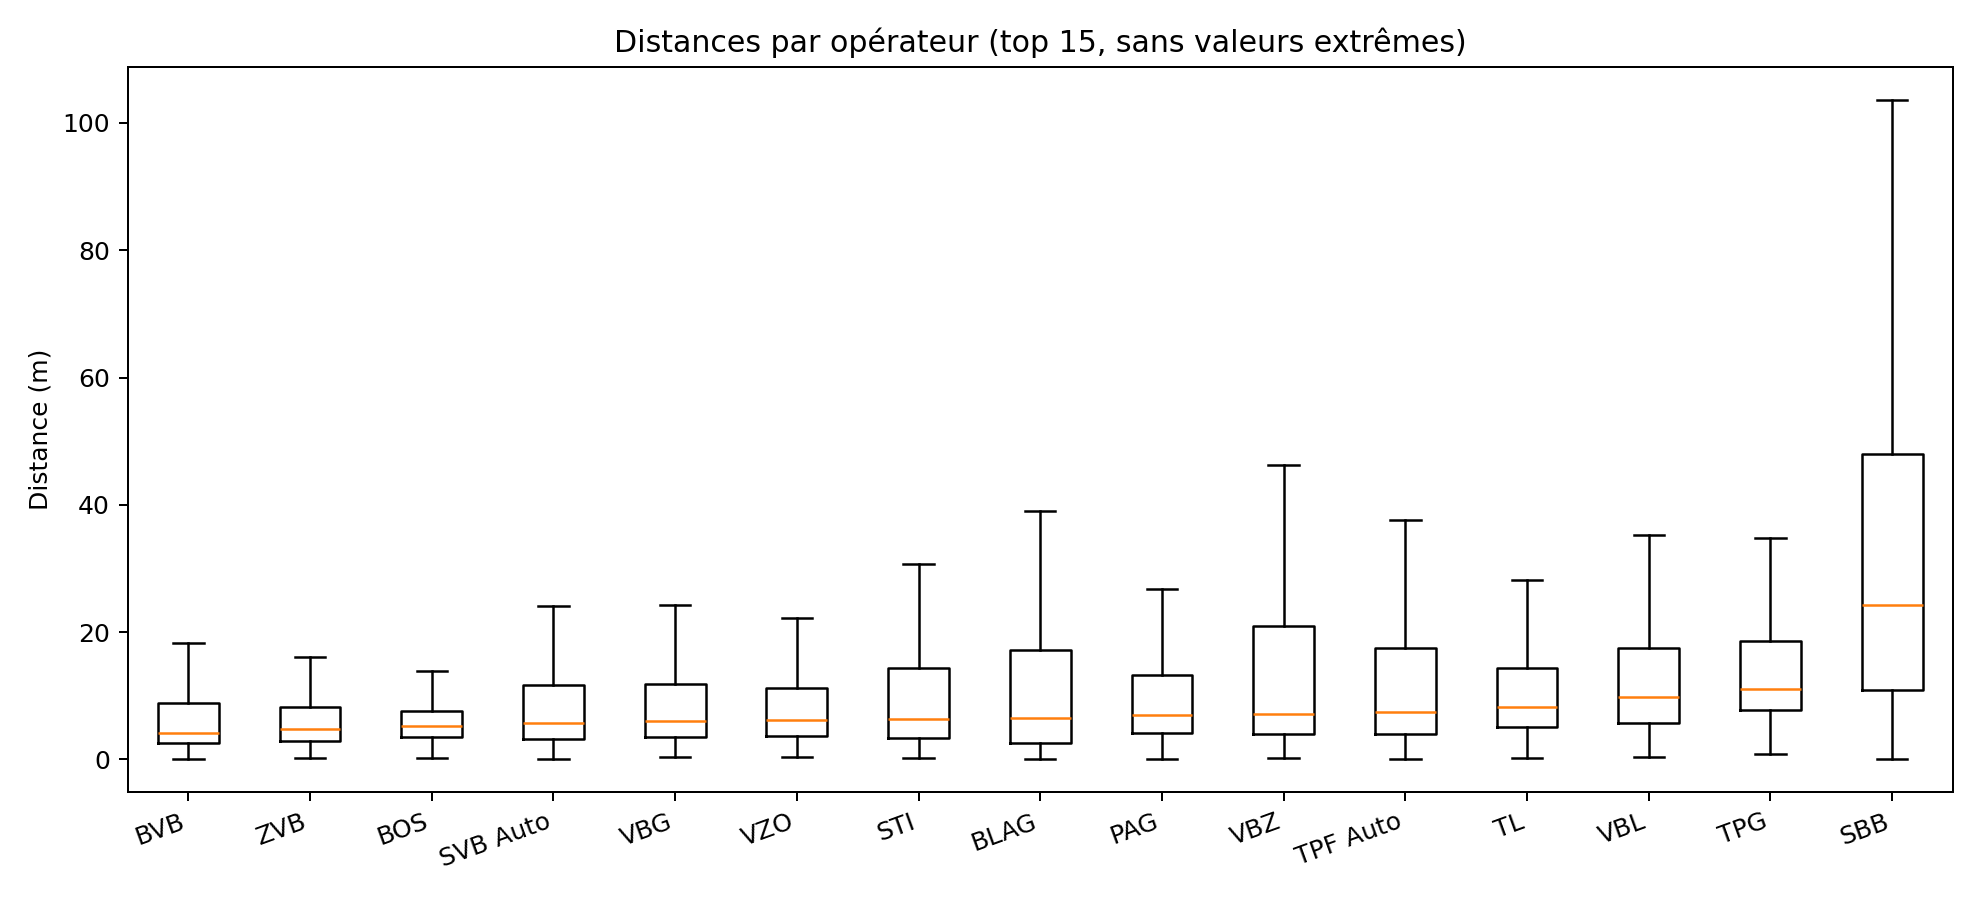
\includegraphics[width=\textwidth]{../figures/chap5/distances_by_operator_box.png}
    \caption[Distances par opérateur]{Dispersion des distances par opérateur (top 15 par effectif).}
\end{figure}

\section{Répartition par tranches de distance}

\begin{figure}[H]
    \centering
    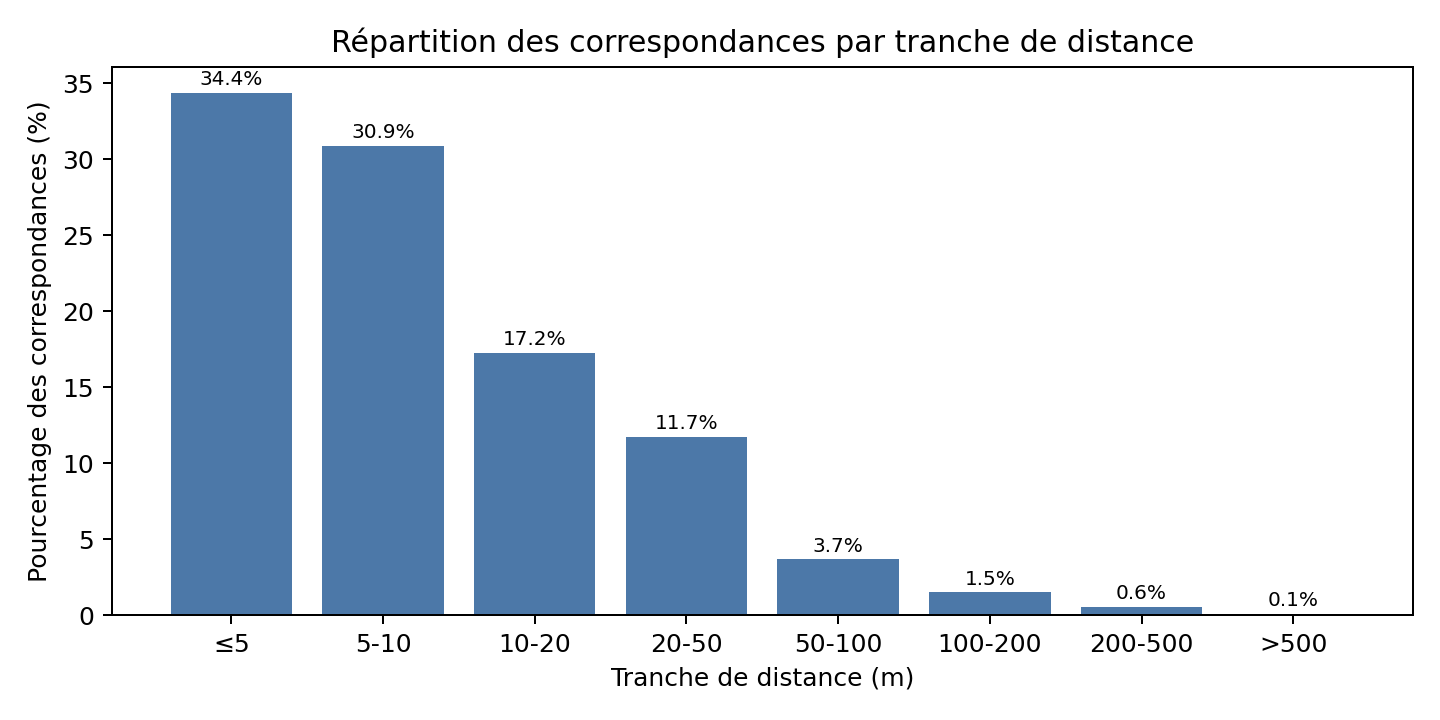
\includegraphics[width=0.9\textwidth]{../figures/chap5/distance_coverage_buckets.png}
    \caption[Tranches de distance]{Part des correspondances sous 5 m, 10 m, 20 m, etc.}
\end{figure}

\section{Cas extrêmes: top 10 plus grandes distances}

Table des 10 plus grandes distances parmi les correspondances, avec désignations officielles ATLAS/OSM, méthode d'appariement, et UIC (ATLAS/OSM).

\begin{table}[H]
    \centering
    % Auto-generated by distance_distributions_and_top10.py
\begin{small}
\begin{minipage}{0.8\textwidth}
\begin{tabularx}{\textwidth}{>{\raggedright\arraybackslash}X >{\raggedright\arraybackslash}X >{\raggedright\arraybackslash}p{2.2cm} >{\raggedright\arraybackslash}p{3.0cm} r}
\toprule
ATLAS (officiel) & OSM (officiel) & Méthode & UIC ATLAS / OSM & \multicolumn{1}{c}{Distance (m)} \\
\midrule
Bex, Les Luisances & Les Plans-sur-Bex, Pont de Nant & Exact (post) & 8570643 / 8570643 & 6650.2 \\
Villars-sur-Ollon, La Roche & Villars-sur-Ollon, La Roche & Exact & 8501707 / 8501707 & 3226.7 \\
Villars-sur-Ollon, La Roche & Villars-sur-Ollon, La Roche & Exact & 8501707 / 8501707 & 3226.6 \\
Col-de-Chassoure (Tortin) & Col-de-Chassoure (Tortin) & Exact & 8530100 / 8530100 & 2487.7 \\
Cabane-des-Violettes & Cabane-des-Violettes & Exact & 8530169 / 8530169 & 1879.0 \\
Espel (Talst.Stöfelibahn) & Espel (Talst.Stöfelibahn) & Exact & 8500277 / 8500277 & 1451.9 \\
Piz Mundaun & Piz Mundaun & Exact & 8530543 / 8530543 & 1413.3 \\
Faido & Faido & Name & 8505204 / 8505204 & 892.9 \\
Diga di Luzzone/Ristorante & Diga di Luzzone/Ristorante & Exact & 8588141 / 8588141 & 846.8 \\
Lutry, Taillepied & Lutry, Taillepied & Exact & 8592163 / 8592163 & 680.1 \\
\bottomrule
\end{tabularx}
\end{minipage}
\end{small}

    \caption[Top 10 distances]{Top 10 des plus grandes distances — repérage des cas à investiguer.}
\end{table}
